\documentclass{beamer}
\usefonttheme{professionalfonts}
\usepackage{amsthm,amssymb,amsmath}
\usepackage{fontspec}
\usepackage{breqn}
\usepackage{tikz}
\usetikzlibrary{decorations.pathreplacing} 
\usepackage{amsmath,amssymb,amsthm,amsfonts}
\usepackage{mathrsfs}
\usepackage{ragged2e}
\usepackage{polyglossia}
\usepackage{graphicx}
\graphicspath{{../images/}}
\theoremstyle{definition}
\newtheorem{definicija}{Definīcija}

\usefonttheme{serif}
\usetheme{Copenhagen}
\setbeamerfont{frametitle}{size=\Large,series=\bfseries}
%\setbeamertemplate{frametitle}[default][center]

%\defbeamertemplate*{title page}{customized}[1][]
%{
%	\centering
%	\small\uppercase{Latvijas Universitāte}\\
%	\small\uppercase{fizikas, matemātikas un optometrijas fakultāte}\\
%	\small\uppercase{Matemātiaks nodaļa}\par
%\vfill
%	\textbf{\large\uppercase{par raupjā integrāļa definīciju}}\\ ~
%
%	\small KURSA DARBS\\
%\vfill
%\begin{flushleft}
%	\usebeamerfont{author}Autors: \textbf{\insertauthor} \\
%	Studenta apliecības Nr.: ek16073 \\
%	Darba vadītājs: profesore Dr. math Svetlana Asmuss\\ ~
%\end{flushleft}	
%~
%
%\hfill RĪGA 2019 \hfill\hfill
%
%}

\title{Par Raupjā integrāļa alternatīvu definīciju}
\author{Emīls Kalugins}
\date{}

\begin{document}
\setbeamertemplate{enumerate item}[default]
\setbeamertemplate{enumerate subitem}[default]

%\setbeamertemplate{footline}{}
\begin{frame}
\maketitle
\end{frame}

%\begin{frame}
%
%\frametitle{Saturs}
%
%
%\begin{enumerate}
%
%\scriptsize
%\item[] Ievads
%\item Šokē integrālis
%\begin{enumerate}
%\scriptsize
%\item Nestriktais mērs
%\item Šokē integrāļa jēdziens 
%\end{enumerate}
%\item Raupjais integrālis 
%\begin{enumerate}
%\scriptsize
%\item Raupjas kopas jēdziens 
%\begin{enumerate}
%\tiny
%\item[] Klasifikācija ar ekvivalences attiecību
%\item[] Atribūti 
%\item[] Informāciju sistēmas 
%\item[] Kopas aproksimācija 
%\end{enumerate}
%\item Raupjais mērs
%\begin{enumerate}
%\tiny
%\item[] Raupjā piederības funkcija
%\end{enumerate}
%\item Šokē integrālis attiecībā pret raupju mēru
%\begin{enumerate}
%\tiny
%\item[] Potenciālie pielietojumi
%\end{enumerate}
%\item Raupjais augšējais un apakšējais integrālis
%\begin{enumerate}
%\tiny
%\item[] Ekvivalenču attiecību virknes
%\item[] Raupjās Darbū summas
%\item[] Raupjie augšējie un apakšējie Darbū integrāļi
%\item[] Raupjais Darbū integrālis
%\end{enumerate}
%\end{enumerate}
%\item[] Nobeigums
%\item[] Izmantotā literatūra un avoti
%\end{enumerate}
%
%\end{frame}

\begin{frame}
\frametitle{Ievads}
\begin{itemize}
\setlength\itemsep{1em}
\item Nestrikto kopu teorijā pastāv labi
attīstīti integrāļi, kā Šokē, Sugeno [1] un Šipoša [2] integrāļi, kuru attīstība sākās jau 1953.
gadā, kad G. Šokē publicēja savu kapacitātes teoriju, ietverot Šokē integrāli [3]. 
\item Raupjo
kopu teorijā tikai salīdzinoši nesen — 2000. gadā J. Peters publicēja pirmo rakstu par
raupjo integrāli, kas balstīts uz Šokē integrāli [4].
\end{itemize}
\end{frame}

\section{Šokē integrālis}

\begin{frame}
\frametitle{Nestriktais mērs}

\begin{definicija}
\footnotesize
  Par $\sigma$\emph{-aditīvu mēru} uz $\sigma$-algebru $\mathfrak{S}$ no kopas
  $S$ apakškopām sauc funkciju $\mu: \mathfrak{S} \rightarrow \mathbb{R}_{\geq
    0}$, kurai ir spēkā
  \begin{enumerate}
  \item $\mu(\emptyset)=0$;
  \item Ja $\{X_n\}_{n\in \mathbb{N}}$ ir kopu saime ar savstarpēji nešķeļošām
    kopām no $\mathfrak{S}$, tad

    $$
    \mu\left( \bigcup_{n=1}^\infty X_n \right) = \sum\limits_{n=1}^\infty\mu(X_n).
    $$
  \end{enumerate}
\end{definicija}


\begin{definicija}
\footnotesize
	Funkciju $\mu : \mathscr{P}(S) \rightarrow \mathbb{R}_{\leq 0}$, kas uzdota uz
  kādas kopas $S$ apakškopām, sauc par \emph{nestriktu mēru}, ja tai izpildās
  sekojošas īpašības:
  \begin{enumerate}
  \item $\mu (\emptyset) = 0$;
  \item Ja $ A \subseteq B$ , tad $\mu(A) \leq \mu(B)$ visiem $A,B \in
    \mathscr{P}(S)$ (\emph{monotonitāte}).
  \end{enumerate}

\end{definicija}
\end{frame}
\begin{frame}
\frametitle{Šokē integrāļa jēdziens}
\begin{definicija}
  Pieņemsim, ka $X$ ir galīga, netukša kopa, kuras elementi ir apzīmēti ar $x_1,
  x_2, \dots ,x_n$. Pieņemsim, ka $\mu$ ir nestrikts mērs uz $\mathscr{P}(S)$.
  Tad Šokē integrālis $C_\mu(f)$ no $f:X \rightarrow [0,1]$ attiecībā pret $\mu$
  tiek definēts kā
  \begin{equation*}
  C_\mu(f) := \sum\limits_{i=1}^n (f(x_{(i)})-f(x_{(i-1)}))\mu(X_{i}),
\end{equation*}
kur $f(x_{(i)})$ apzīmē to, ka indeksi ir permutēti tā, lai $0 \leq
  f(x_{(1)})\leq \cdots \leq f(x_{(n)})$, bet $ X_{(i)} =
  {\{x_{(i)},x_{(i+1)},\dots,x_{(n)}\}}$ un $f(x_{(0)}) = 0$.

\end{definicija}
\end{frame}
\begin{frame}
\frametitle{Grafiskā interpretācija}
\begin{figure}
		\centering
	\begin{tikzpicture}[scale=0.85]
		\draw[->] (0,0) -- (8,0);
		\draw[->] (0,0) -- (0,6);
		\node[anchor=east,align=right] at (0,1.2) {$f(x_{(1)})$};
		\node[anchor=east,align=right] at (0,2.5) {$f(x_{(2)})$};
		\node[anchor=east,align=center] at (-0.5,3.3) {$\vdots$};
		\node[anchor=east,align=right] at (0,4) {$f(x_{(n-1)})$};
		\node[anchor=east,align=right] at (0,5) {$f(x_{(n)})$};

		\draw[black] (0,5) -- (0.8,5) -- (0.8,0);
		\draw[black] (0,4) -- (2.6,4) -- (2.6,0);
		\draw[black] (0,2.5) -- (5.0,2.5) -- (5.0,0);
		\draw[black] (0,1.2) -- (6.9,1.2) -- (6.9,0);

		\node[anchor=north] at (0.8,0) {$\mu(X_{(n)})$};
		\node[anchor=north] at (2.6,0) {$\mu(X_{(n-1)})$};

		\node[anchor=north] at (3.9,-0.1) {$\cdots$};
		\node[anchor=north] at (5.0,0) {$\mu(X_{(2)})$};


		\node[anchor=north] at (6.9,0) {$\mu(X_{(1)})$};

	\end{tikzpicture}
\end{figure}


\end{frame}

\begin{frame}
\frametitle{Grafiskā interpretācija aditīva mēra gadījumā}
\begin{figure}
	\begin{tikzpicture}[scale=0.85]

		\draw[->] (0,0) -- (8,0);
		\draw[->] (0,0) -- (0,6);
		\draw (1.5,0.1) -- (1.5,-0.1);
		\draw (1.0,0) -- (1.0,4) -- (2.0,4) -- (2.0,0);
		\draw[decorate,decoration={brace,mirror,amplitude=3pt},yshift=-10pt] (1.0,0) -- (2.0,0) node [black,midway,yshift=-12pt] {\footnotesize $\mu(\{x_1\})$};

		\node[anchor=north] at (1.5,0) {$x_1$};
		\node[anchor=south] at (1.5,4) {$f(x_1)$};

		\draw (3,0.1) -- (3,-0.1);
		\draw (2.0,0) -- (2.0,2.4) -- (4.0,2.4) -- (4.0,0);
		\draw[decorate,decoration={brace,mirror,amplitude=3pt},yshift=-10pt] (2.0,0) -- (4.0,0) node [black,midway,yshift=-12pt] {\footnotesize $\mu(\{x_2\})$};

		\node[anchor=north] at (3.0,0) {$x_2$};
		\node[anchor=south] at (3.0,2.4) {$f(x_2)$};
		\node[anchor=north] at (5,0) {$\cdots$};

		\node[anchor=north] at (6.5,0) {$x_n$};
		\node[anchor=south] at (6.5,3.3) {$f(x_n)$};

		\draw (6.5,0.1) -- (6.5,-0.1);

		\draw (5.8,0) -- (5.8,3.3) -- (7.2,3.3) -- (7.2,0);
		\draw[decorate,decoration={brace,mirror,amplitude=3pt},yshift=-10pt] (5.8,0) -- (7.2,0) node [black,midway,yshift=-12pt] {\footnotesize $\mu(\{x_n\})$};

	\end{tikzpicture}

\end{figure}

\end{frame}

\section{Raupjais integrālis}

\begin{frame}
\frametitle{Raupjas aproksimācijas}
\begin{definicija}
  Kopai $X \subseteq U$ no universa $U$ ar ekvivalences attiecību $R$ par
  $R$-\emph{apakšējo aproksimāciju} un $R$-\emph{augšējo aproksimāciju}
  attiecīgi sauc kopas $\underline{R}X$ un $\overline{R}X$, kas definētas kā
\begin{align*}
  \underline{R}X = \{x \in U  : [x]_R \subseteq X\},\\
  \overline{R}X = \{x \in U : [x]_R \cap X \neq \emptyset\}.
\end{align*}
\end{definicija}
\end{frame}

\begin{frame}
\frametitle{Raupjo aproksimāciju interpretācija}
  \centering
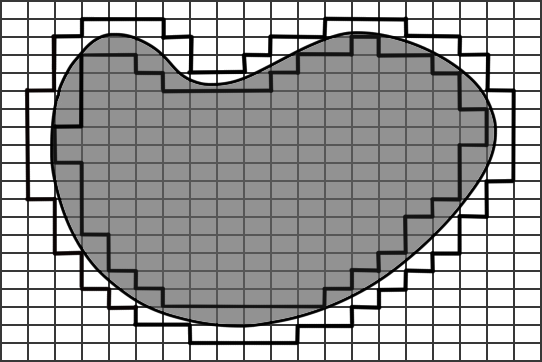
\includegraphics[width=0.9\textwidth]{raupjaaproks} 
\end{frame}
\begin{frame}
\begin{definicija}
\frametitle{Raupjais mērs}
Pieņemsim, ka $X \subseteq U, R$ ir ekvivalences attiecība uz $U$,
un ${u \in U}$. Pieņemsim, ka $\rho' : \mathscr{P}(X) \rightarrow \mathbb{R}_{\geq
0}$ ir aditīvs mērs uz $\mathscr{P}(X)$. Tad funkciju ${\rho_u : \mathscr{P}(S)
\rightarrow \mathbb{R}_{\geq 0}}$, kas definēta kā $\rho_u(Y) = \rho'(Y\cap
[u]_R)$ katram $Y \in \mathscr{P}(X)$, sauc par \emph{raupju mēru} attiecībā pret
faktorkopu $U/R$ un objektu $u$.
\end{definicija}
\end{frame}

\begin{frame}
\frametitle{Šokē integrālis attiecībā pret raupju mēru}
\begin{definicija}[{[5]}]
Pieņemsim, ka $\rho$ ir raupjš mērs uz kopu $X$, kura elementus varam apzīmēt ar
$x_1,x_2,\dots,x_n$. \emph{Raupjais diskrētais integrālis} no funkcijas
$f:X\rightarrow \mathbb{R}_{\geq 0}$ attiecībā pret raupjo mēru $\rho$ tiek
definēts kā
\begin{equation} \label{eq:raupj}
  \int_Xf\;d\rho := \sum_{i=1}^n(f(x_{(i)})-f(x_{(i-1)}))\rho(X_{(i)}),
\end{equation}
kur $f(x_{(i)})$ apzīmē to, ka indeksi ir permutēti tā, lai $0 \leq
  f(x_{(1)})\leq \cdots \leq f(x_{(n)})$, bet $ X_{(i)} =
  {\{x_{(i)},x_{(i+1)},\dots,x_{(n)}\}}$ un $f(x_{(0)}) = 0$.
\end{definicija}
\end{frame}

\begin{frame}
\frametitle{Potenciālie pielietojumi}

\begin{itemize}
\setlength\itemsep{3em}
\item Noteiktos gadījumos diskrētais raupjais integrālis spēj aproksimēt eksperta lēmumu.
\item Vai ir iespējams noteikt īpašību, kura bija noteicošā eksperta lēmumā?
\end{itemize}
\end{frame}

\begin{frame}
\frametitle{Ekvivalenču attiecību virknes}
\begin{definicija}
  Ekvivalenču attiecību virkni $\{R_n\}_{n\in\mathbb{N}}$ sauksim par
  \emph{konverģējošu ekvivalenču attiecību nozīmē}, ja
  $$
\lim\limits_{n\rightarrow \mathbb{N}} R_n(x,y) = 1 \iff x = y 
  $$

\end{definicija}

\begin{definicija}
  Ekvivalences attiecība $R'$ \emph{sasmalcina} ekvivalences attiecību $R$, ja 
  $$
  R' \cap R = R'.
  $$
\end{definicija}
\end{frame}

\begin{frame}
\frametitle{Raupjās Darbū summas}
\begin{definicija}
  Par \emph{raupjo augšējo Darbū summu} attiecībā pret ekvivalences attiecību
  $R_n$, mēru $\mu$ un funkciju $f$ sauksim izteiksmi
  $$
  U(R_n,f) = \sum\limits_{[x_i]\in\mathscr{R}(\overline{R_n}X)} \sup\limits_{x \in
    [x_i]} f(x) \; \mu{([x_i])}.
  $$

\end{definicija}

\begin{definicija}
Par \emph{raupjo apakšējo Darbū summu} attiecībā pret ekvivalences attiecību
  $R_n$, mēru $\mu$ un funkciju $f$ sauksim izteiksmi
  $$
  L(R_n,f) = \sum\limits_{[x_i]\in\mathscr{R}(\underline{R_n}X)} \inf\limits_{x \in
    [x_i]} f(x) \; \mu{([x_i])}.
  $$
\end{definicija}

\end{frame}

\begin{frame}
\frametitle{Raupjie augšējie un apakšējie Darbū integrāļi}
\begin{definicija}
Par \emph{raupjo augšējo Darbū integrāli} attiecībā pret ekvivalences attiecību virkni
  $\{R_n\}_{n\in\mathbb{N}}$, mēru $\mu$ un funkciju $f$ sauksim izteiksmi
  $$
  (\mathcal{R}) \; U_f = \inf\limits_{n\in\mathbb{N}} U(R_n,f).
  $$
\end{definicija}


\begin{definicija}
Par \emph{raupjo apakšējo Darbū integrāli} attiecībā pret ekvivalences attiecību
  virkni $\{R_n\}_{n\in\mathbb{N}}$, mēru $\mu$ un funkciju $f$ sauksim izteiksmi
  $$
  (\mathcal{R}) \; L_f = \sup\limits_{n\in\mathbb{N}} L(R_n,f).
  $$
\end{definicija}
\end{frame}
\begin{frame}
\frametitle{Nobeigums}
\begin{itemize}
\setlength\itemsep{2em}
\item Darbā izklāstīta pašreizējā diskrētā raupjā integrāļa attīstība un definīcija, piedāvājot alternatīvu definīciju, attālinoties no Šokē integrāļa.
\item Ņemot vērā, ka raupjais integrālis varētu spēlēt lomu lēmumu pieņemšanā un nav attīstītas teorijas par integrāļiem raupjās kopās, jāturpina pētīt iespējamās integrāļa definīcijas un to īpāšības, kas balstās uz raupjām kopām. 
\end{itemize}
\end{frame}

\begin{frame}
\frametitle{Izmantotā literatūra un avoti}
\small
[1] V. Torra and Y. Narukawa, “The interpretation of fuzzy integrals and their appli-
cation to fuzzy systems,” \textit{International Journal of Approximate Reasoning}, vol. 41,
no. 1, pp. 43–58, 2006. \\~


[2] J. Šipoš, “Integral with respect to a pre-measure,” \textit{Mathematica Slovaca}, vol. 29,
no. 2, pp. 141–155, 1979.\\~


[3] G. Choquet, “Theory of capacities,” in \textit{Annales de l’institut Fourier}, vol. 5, pp. 131–
295, 1954.\\~


[4] J. Peters, L. Han, and S. Ramanna, “The choquet integral in a rough software cost
estimation system,” \textit{Studies in Fuzziness and Soft Computing}, vol. 40, pp. 392–414,
01 2000.\\~


[5] Z. Pawlak, J. F. Peters, A. Skowron, Z. Suraj, S. Ramanna, and M. Borkowski,
\textit{Rough Measures, Rough Integrals and Sensor Fusion}, pp. 263–272. Berlin, Heidelberg:
Springer Berlin Heidelberg, 2003. 
\end{frame}

\begin{frame}
\frametitle{Izmantotā literatūra un avoti}
\small
[6] K. Hrbacek. and T. Jech, \textit{Introduction to set theory}. M. Dekker New York, 1999.\\~

[7] M. Grabisch, “The application of fuzzy integrals in multicriteria decision making,”
European journal of operational research, vol. 89, no. 3, pp. 445–456, 1996.\\~

[8] Z. Pawlak, “Rough sets,” \textit{International Journal of Computer \& Information Sciences},
vol. 11, pp. 341–356, Oct 1982.\\~

[9] Z. Pawlak, “Information systems theoretical foundations,” \textit{Information systems},
vol. 6, no. 3, pp. 205–218, 1981.\\~

[10] P. Pattaraintakorn, J. Peters, and S. Ramanna,\textit{ Capacity-Based Definite Rough Integral and Its Application}, vol. 59, pp. 299–308. 10 2009.
\end{frame}
\end{document}
